\newpage
\section{Bitmaps bewegen}\index{Bitmap!bewegen}
\subsection{Grundlagen}
In der Zusammenfassung des vorherigen Kapitels haben wir für die Darstellung von Bitmaps notiert, dass wir die linke, obere Ecke als Positionsangabe und die Höhe und Breite beispielsweise für Abstandsberechnungen brauchen. Diese Angaben lassen sich gut einem Rechteck kodieren. Pygame stellt dazu die Klasse \texttt{pygame.rect.Rect}\myindex{pyg}{\texttt{Rect}}\randnotiz{Rect} zur Verfügung. In \abbref[vref]{picRect01} finden Sie die meiner Ansicht nach wichtigsten Attribute der Klasse.

\begin{figure}[H]
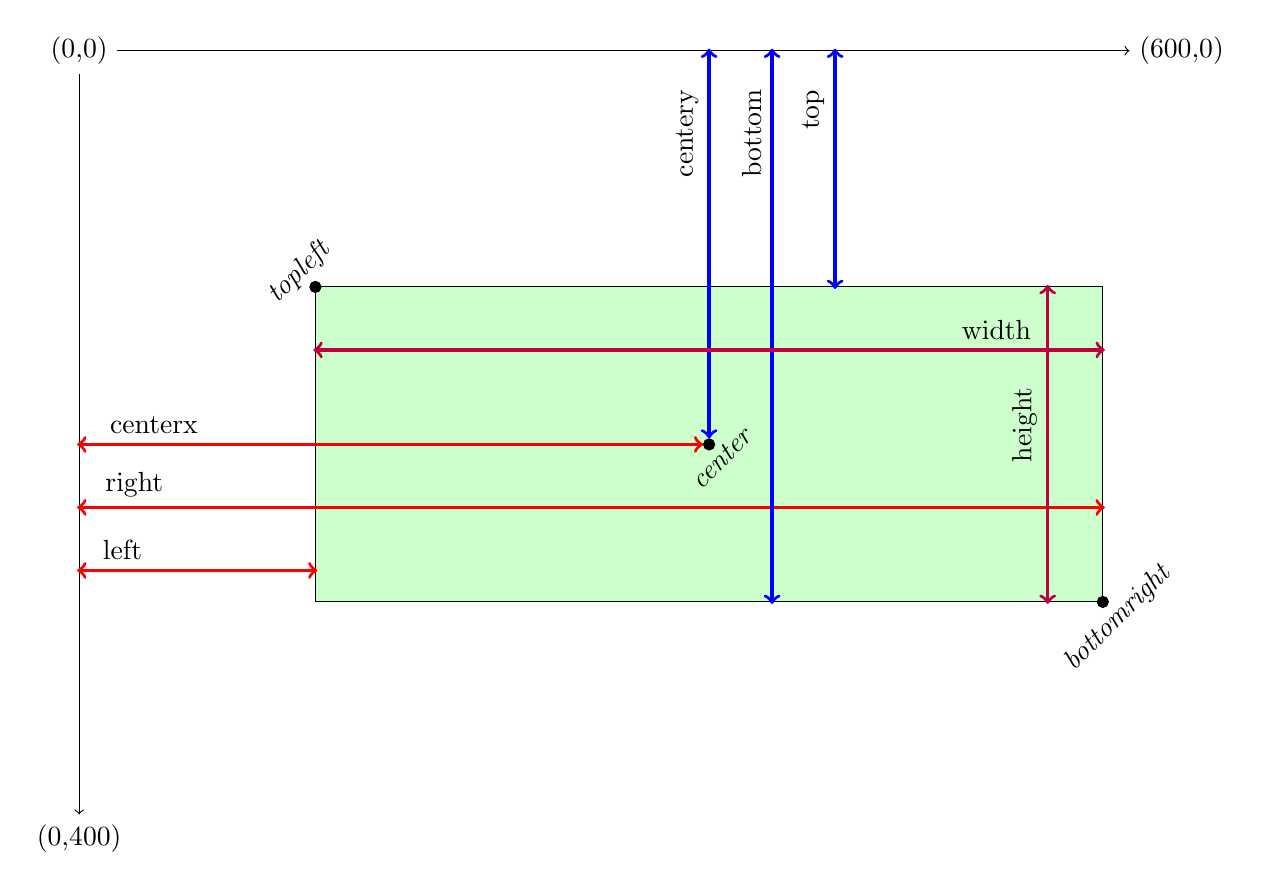
\begin{tikzpicture}
%Bildschirm Koordinatensystem
\draw
 (0,10) node (o) {(0,0)}
 (0,0) node (y) {(0,400)}
 (14,10) node (x) {(600,0)}
;
\draw[->] (o) -- (x);
\draw[->] (o) -- (y);

%Rechteck
\draw
 (3,7) node (topleft) {}
 (13,3) node (bottomright) {}
 (8.0,5) node (centerxy) {}
;
\filldraw[fill=green!20] (topleft) rectangle (bottomright);
\draw (topleft) node[above, rotate=45] {\emph{topleft}};
\draw (bottomright) node[below, rotate=45] {\emph{bottomright}};
\filldraw[fill=black] (centerxy) circle (2pt) node[below, rotate=45] {\emph{center}};
\filldraw[fill=black] (topleft) circle (2pt);
\filldraw[fill=black] (bottomright) circle (2pt);

%Left
\draw
 (-0.15,3.4) node (left1) {}
 (3.15,3.4) node (left2) {}
;
\draw[<->, very thick, red] (left1) -- (left2) node[above, black, xshift=-2.6cm] {left};


%Right
\draw
 (-0.15,4.2) node (right1) {}
 (13.15,4.2) node (right2) {}
;
\draw[<->, very thick, red] (right1) -- (right2) node[above, black, xshift=-12.45cm] {right};

%Centerx
\draw
 (-0.15,5.0) node (cx1) {}
 (8.05,5.0) node (cx2) {}
;
\draw[<->, very thick, red] (cx1) -- (cx2) node[above, black, xshift=-7.1cm] {centerx};

%top
\draw
 (9.6,10.15) node (top1) {}
 (9.6,6.85) node (top2) {}
;
\draw[<->, very thick, blue] (top1) -- (top2) node[above, black, yshift=2.4cm, rotate=90] {top};

%bottom
\draw
 (8.8,10.15) node (bottom1) {}
 (8.8,2.85) node (bottom2) {}
;
\draw[<->, very thick, blue] (bottom1) -- (bottom2) node[above, black, yshift=6.1cm, rotate=90] {bottom};

%Centery
\draw
 (8.0,10.15) node (cy1) {}
 (8.0,4.95) node (cy2) {}
;
\draw[<->, very thick, blue] (cy1) -- (cy2) node[above, black, yshift=4cm, rotate=90] {centery};

%Width
\draw
 (2.85,6.2) node (w1) {}
 (13.15,6.2) node (w2) {}
;
\draw[<->, very thick, purple] (w1) -- (w2) node[above, black, xshift=-1.5cm] {width};

%height
\draw
 (12.3,7.15) node (h1) {}
 (12.3,2.85) node (h2) {}
;
\draw[<->, very thick, purple] (h1) -- (h2) node[above, black, yshift=2.4cm, rotate=90] {height};

\end{tikzpicture}
\caption{Elemente eines \texttt{Rect}-Objekts}\label{picRect01}
\end{figure}

\myindex{pyg}{\texttt{Rect}!\texttt{centerx}}%
\myindex{pyg}{\texttt{Rect}!\texttt{right}}%
\myindex{pyg}{\texttt{Rect}!\texttt{left}|underline}%
\myindex{pyg}{\texttt{Rect}!\texttt{centery}}%
\myindex{pyg}{\texttt{Rect}!\texttt{bottom}}%
\myindex{pyg}{\texttt{Rect}!\texttt{top}|underline}%
\myindex{pyg}{\texttt{Rect}!\texttt{topleft}}%
\myindex{pyg}{\texttt{Rect}!\texttt{bottomright}}%
\myindex{pyg}{\texttt{Rect}!\texttt{center}|underline}%
\myindex{pyg}{\texttt{Rect}!\texttt{width}|underline}%
\myindex{pyg}{\texttt{Rect}!\texttt{height}|underline}%
In der Abbildung werden Strecken in normaler Schrift und Punkte in \textit{kursiver Schrift} angegeben. Die Strecken sind eindimensional und die Punkte zweidimensional $(x,y)$. Die Koordinate~$x$ ist dabei der horizontale und~$y$ der vertikale Abstand zum 0-Punkt des Koordinatensystems. Die Bedeutung der einzelnen Angaben sollte selbsterklärend sein. Der schöne Vorteil ist, dass die Angaben sich gegenseitig berechnen. Setze ich beispielsweise \texttt{topleft = (10,10)} und \texttt{width, height = 30, 40}, so werden alle anderen Angaben für mich ermittelt. Ich muss also nicht mehr den rechten Rand mit \texttt{left + width} ausrechnen; ich kann vielmehr sofort \texttt{right} verwenden. Auch oft nützlich ist die Berechnung des Mittelpunktes \texttt{center} oder die entsprechenden Längen \texttt{centerx} und \texttt{centery}. Ändere ich nun das Zentrum durch \texttt{center = (100, 10)}, so verschieben sich alle anderen Angaben ebenfalls und müssen nicht von mir neu bestimmt werden -- sehr praktisch.

Schauen wir uns dazu eine reduzierte Version des letzten Quelltextes an. In \srcref[vref]{srcInvader05} wird die \texttt{Rect}-Klasse schon verwendet. So werden beispielsweise in \zeiref{srcInvader0504a} die Fenstermaße in einem \texttt{Rect}-Objekt verwaltet. In den Zeilen \zeiref{srcInvader0504b}, \zeiref{srcInvader0502} und \zeiref{srcInvader0503} können dadurch die Bildschirminformationen bequem und ohne eigene Berechnungen ausgelesen werden.

\lstsource{SRC/00 Einführung/04 Bewegung/invader05.py}{1}{999}{python}{Bitmaps bewegen, Version 1.0}{srcInvader05}

Für \texttt{Surface}-Objekte können wir sehr bequem mit \texttt{pygame.Surface.get\_rect()}\myindex{pyg}{\texttt{Surface}!\texttt{get\_rect()}}\randnotiz{get\_rect()} das \texttt{Rect}-Objekt erstellen lassen (\zeiref{srcInvader0501}). Die Positionierung kann nun leichter über die Attribute erfolgen. Das Zentrum muss beispielsweise nicht mehr in die Berechnung einfließen, ich kann vielmehr das horizontale Zentrum direkt als halbe Fensterbreite festlegen (\zeiref{srcInvader0502}). Auch muss die vertikale Koordinate nicht mehr vom oberen Rand aus betrachtet werden, sondern ich kann viel intuitiver den Abstand des unteren Randes vom Bildschirmrand angeben (\zeiref{srcInvader0503}). Und als Sahnehäubchen kann das \texttt{Rect}-Objekt auch noch als Parameter der \randnotiz{blit()}\myindex{pyg}{\texttt{Surface}!\texttt{blit()}}\texttt{blit()}-Funktion übergeben werden (\zeiref{srcInvader0504}).

\myebild{invader05.png}{0.8}{Bitmaps bewegen, Version 1.0}{picInvader05}

Das Ergebnis ist unspektakulär (siehe \abbref[vref]{picInvader05}) und hat noch nichts mit Bewegung zu tun.

Bewegung wird in Spielen durch veränderte Positionen animiert. Soll das Raumschiff sich nach rechts bewegen, muss sich daher die horizontale Koordinate des Schiffs erhöhen. Welche horizontale Koordinate Sie dazu verwenden -- \texttt{left}, \texttt{right} oder \texttt{centerx} --, können Sie von ihrer Spiellogik abhängig machen. In unserem Beispiel ist das egal; ich nehme daher \texttt{left}.

\lstset{firstnumber=38}
\begin{lstlisting}
defender_rect.left = defender_rect.left + 1
\end{lstlisting}

Allein diese kleine Ergänzung lässt unser Raumschiff nun nach rechts wandern. Die \texttt{+1} kodiert dabei zwei Informationen: 
\begin{itemize}
	\item \textbf{Richtung:}\randnotiz{Richtung}\index{Richtung} Hier ist das Vorzeichen \texttt{+}. Dadurch erhöht sich die Angabe \texttt{left} bei jedem Schleifendurchlauf; der linke Rand der Grafik wandert damit nach rechts. Wollte man nach links wandern, müsste das Vorzeichen ein~\texttt{-} sein. Die horizontale Koordinate wird dadurch immer kleiner und nähert sich damit der~0. Völlig analog würde das Vorzeichen die Richtung in der Vertikalen steuern. Ein~\texttt{+} würde die Grafik nach unten und ein~\texttt{-} nach oben bewegen. Probieren Sie es aus!
	
	\item \textbf{Geschwindigkeit:}\randnotiz{Ge\-schwin\-dig\-keit}\index{Geschwindigkeit} Die \texttt{1} legt fest, um welche Größenordnung sich \texttt{left} verändert. Je größer der Wert ist, desto größer sind die Sprünge zwischen den Frames; die Bewegung erscheint schneller. 
\end{itemize}

\lstsource{SRC/00 Einführung/04 Bewegung/invader05b.py}{24}{40}{python}{Bitmaps bewegen, Version 1.2}{srcInvader05b}

Diese beiden Informationen werden nun in \srcref[vref]{srcInvader05b} dazu genutzt, die Bewegung erheblich flexibler zu gestalten. In \zeiref{srcInvader0505} die Geschwindigkeit nun durch die Variable \texttt{defender\_speed} repräsentiert. So könnten wir im Laufe des Spiels die Geschwindigkeit dynamisch gestalten, z.B. bei einer Beschleunigung durch Raketentreibstoffausstoß. 

Die Richtung wird in \zeiref{srcInvader0506} ebenfalls in einer Variablen abgelegt: \texttt{defender\_direction}. Derzeit ist sie positiv, aber wir werden schon bald sehen, dass wir diese auch für Richtungswechsel nutzen können.

Beide Informationen können nun in \zeiref{srcInvader0507} zur Berechnung der neuen horizontalen Position genutzt werden.

Wenn Sie das Programm laufen lassen, verabschiedet sich der Verteidiger nach einiger Zeit und verschwindet hinter dem rechten Bildschirmrand und ward nicht mehr gesehen. Nutzen wir nun unser Rechteck zu einer ersten einfachen Kollisionsprüfung. Ich möchte, dass das Raumschiff von den Rändern \emph{abprallt} und die Richtung wechselt. 

\lstsource{SRC/00 Einführung/04 Bewegung/invader05c.py}{35}{40}{python}{Bitmaps bewegen, Version 1.3}{srcInvader05c}

Ich hoffe, dass Sie die Idee hinter dem Code erkennen. Nach Berechnung der neuen horizontalen Position, wird in \zeiref{srcInvader0508} überprüft, ob der neue rechte Rand des Bitmaps die rechte Bildschirmseite erreicht oder überschreitet. Wenn ja, dann wird einfach das Vorzeichen der Richtungsvariable vertauscht\index{Richtungswechsel}\randnotiz{Rich\-tungs\-wechs\-el}! Analog klappt das beim Erreichen des linken Bildschirmrandes. 

Probieren Sie doch mal aus, das Ganze mit einer vertikalen Bewegung zu kombinieren.

Ein Problem habe ich noch: In \zeiref{srcInvader0507} wird die neue Position dem \texttt{Rect-}Objekt zugewiesen, obwohl sie vielleicht schon über den Rand ragt. Bei einer Geschwindigkeit von~\texttt{1} oder \texttt{2} mag das nicht so ins Auge fallen, aber wenn wir die Geschwindigkeit auf die Raumschiffbreite einstellen, wird das Problem offensichtlich (setzen Sie kurzfristig mal \texttt{Settings.FPS = 5}, damit man was sieht). Das Raumschiff verlässt zur Hälfte den Bildschirm. 

Wir sollten somit die neue Position überprüfen und erst dann diese dem \texttt{Rect}-Objekt \texttt{defender\_rect} zuweisen. Führen wir in diesem Zusammenhang eine recht nützliche Methode der \texttt{Rect}-Klasse ein: \texttt{pygame.Rect.move()}\myindex{pyg}{\texttt{Rect}!\texttt{move()}|underline}\randnotiz{move()}.

\lstsource{SRC/00 Einführung/04 Bewegung/invader05d.py}{35}{42}{python}{Bitmaps bewegen, Version 1.4}{srcInvader05d}

Die neue Funktion taucht in \zeiref{srcInvader0510} zum ersten Mal auf. Sie hat zwei Parameter. Mit dem ersten wird die Verschiebung der horizontalen Koordinate angegeben und mit der zweiten die vertikale Verschiebung. Da wir keine Höhenposition ändern wollen, ist dieser Parameter in unserem Beispiel konstant~0. Als Rückgabe liefert die Funktion ein neues \texttt{Rect}-Objekt mit den neuen Positionsangaben. Dieses speichern wir in \texttt{newpos} zwischen.

Die nachfolgenden Kollisionsprüfungen werden dann mit dem \texttt{newpos}-Rechteck durchgeführt. Bei einer Kollision werden wie eben die Richtungswerte verändert. Falls keine Kollision mit dem Rand vorliegt, wird \texttt{newpos} zu unserem neuen Rechteck für den Verteidiger (\zeiref{srcInvader0511}).

Wenn Sie jetzt das Programm ausführen, wird die Position bei einer Kollision eben nicht verändert, sondern erst im nächsten Frame.

\begin{figure}[H]
\begin{center}
\begin{tikzpicture}
\node (myfirstpic) at (0,0) {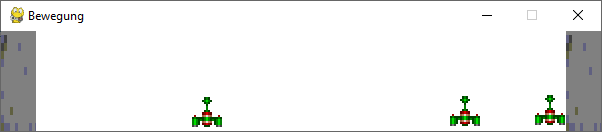
\includegraphics[scale=0.8]{invader06.png}};

\draw
 (-1.8cm,-1.3cm) node (a) {}
 (5.8cm,-1.3cm) node (b) {}
 (5.8cm,-0.57cm) node (c) {}
 (3.4cm,-0.57cm) node (d) {}
;
\draw[>->, very thick, red, densely dotted] (a) -- (b) ;
\draw[>->, very thick, red, densely dotted] (c) -- (d) ;

%node[above, black, xshift=-2.6cm] {move left}
%\draw[->] (a) -- (b);
%\draw[->] (o) -- (y);


%Left
%\draw
% (-0.15,3.4) node (left1) {}
% (3.15,3.4) node (left2) {}
%;
%
\end{tikzpicture}
\caption{Der Verteidiger bewegt sich und prallt ab}\label{picBewegung01}
\end{center}
\end{figure}

%%%%%%%%%%%%%%%%%%%%%%%%%%%%%%%%%%%%%%%%%%%%%%%%%%%%%%%%%%%%%%%%%%%%%%%%%%%%%%%%
\subsection{Geschwindigkeiten normalisieren (\emph{deltatime})}\index{deltatime}
Die Bewegung ist derzeit nicht nur von \texttt{defender\_speed} abhängig, sondern auch von der Framerate \texttt{Settings.FPS}. Um diese Abhängigkeit zu verdeutlichen, habe ich den vorherigen Quelltext für ein kleines Experiment umgebaut (siehe \srcref[vref]{srcInvader05e}).

In \zeiref{srcInvader05e01} sehen Sie die unterschiedlichen Frameraten, mit denen das Experiment durchgeführt wurde. In der Zeile davor werden die Fenstermaße so eingestellt, dass das Fenster hoch und schmal ist, und in der Zeile darunter wird die absolute Anzahl der Millisekunden angegeben, die das Raumschiff nach oben steigt.

\zeiref{srcInvader05e02} merkt sich die Zeit, wann das Aufsteigen des Raumschiffs begonnen hat. Dazu liefert mir die Funktion \texttt{pygame.time.get\_ticks()}\myindex{pyg}{\texttt{time}!\texttt{get\_ticks()}}\randnotiz{get\_ticks()} die Anzahl der Millisekunden seit dem Aufruf von \texttt{pygame.init()}\myindex{pyg}{\texttt{init()}}; also beispielsweise~$5~ms$.

Innerhalb der Hauptprogrammschleife wandert das Raumschiff nun pro Frame eine gewisse Anzahl von Pixel nach oben. Dabei wird die neue Position dadurch ermittelt, dass auf die \texttt{top}-Koordinate der alten Position das Produkt aus Richtung und Geschwindigkeit addiert wird (\zeiref{srcInvader05e03}) -- also nix Neues an dieser Stelle.

Nach einer festen Zeitspanne (\texttt{Settings.LIMIT}, hier $500~ms$) wird die Richtung in \texttt{defender\_direction} auf~0 gesetzt, so dass die Bewegung stoppt. Dazu wird in \zeiref{srcInvader05e04} abgefragt, ob die aktuelle Anzahl von Millisekunden seit dem Start des Programmes größer als \texttt{start\_time} plus \texttt{Settings.LIMIT} ist. Oder in Zahlen: Beim ersten Schleifendurchlauf (Frame~1) stünde dort beispielsweise die Abfrage \emph{Sind $17~ms$ größer als $5~ms + 500~ms$}. Die Antwort ist \emph{Nein}, so dass das Raumschiff sich nach oben bewegt. Bei Frame~61 stünde dort die Abfrage \emph{Sind $508~ms$ größer als $5~ms + 500~ms$}. Nun ist die Antwort \emph{Ja} und die Richtungsvariable wird deshalb auf~0 gesetzt, die Bewegung stoppt.

\lstsource{SRC/00 Einführung/04 Bewegung/invader05e.py}{7}{53}{python}{Nicht normalisierte Bewegung}{srcInvader05e}

In \abbref[vref]{fpsbewegung00} können Sie Bildschirmfotos der Strecken sehen, die das Raumschiff nach einer halben Sekunde zurückgelegt hat. In allen Experimenten blieb die Geschwindigkeit \texttt{defender\_speed} immer gleich -- nämlich 2. Nur die Framerate hat sich erhöht.

Wie kommen diese unterschiedlichen Höhen zustande? Soll doch eigentlich nur \texttt{de\-fen\-der\-\_speed} die Geschwindigkeit definieren. In \tabref[vref]{tabFpsBewegung01} wird der Zusammenhang hoffentlich deutlich. In der ersten Spalte ist die Geschwindigkeit eines Objektes zu sehen; in unserem Beispiel ist dies die Variable \texttt{defender\_speed}. Dieser Wert gibt an, um wie viele Pixel pro Frame das Objekt bewegt wird; dieser Wert wird nicht verändert. Die zweite Spalte gibt die Framerate an, also die Anzahl der Frames pro Sekunde. In unserem Beispiel ist dieser Wert in \texttt{Settings.FPS} definiert. Die Dauer der Bewegung ist in der dritten Spalte zu sehen. Wir haben eine Dauer von $500~ms$ also $0.5~s$. In unserem Beispiels liegt der Wert in \texttt{Settings.LIMIT} und ist ebenfalls für alle Experimente gleich. 

In der letzten Spalte steht die errechnete Wegstrecke in Pixel, die das bewegliche Objekt dann zurückgelegt hat. Nun ist Zusammenhang klar: Da wir die Hauptprogrammschleife wegen der unterschiedlichen Framerate unterschiedlich oft wiederholen, wird bei konstanter Zeit eine unterschiedliche Strecke zurückgelegt.

\begin{figure}[hbtp] 
\begin{center}
\begin{tikzpicture}
\node (fps010) at (0.0, 0) {\fbox{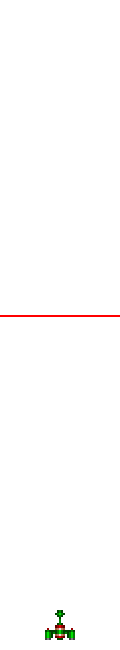
\includegraphics[scale=0.35]{fps_05e_010_00.png}}};
\node (fps030) at (2.0, 0) {\fbox{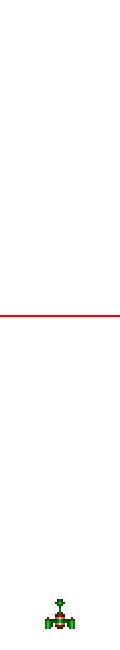
\includegraphics[scale=0.35]{fps_05e_030_00.png}}};
\node (fps060) at (4.0, 0) {\fbox{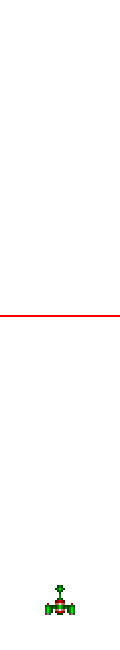
\includegraphics[scale=0.35]{fps_05e_060_00.png}}};
\node (fps120) at (6.0, 0) {\fbox{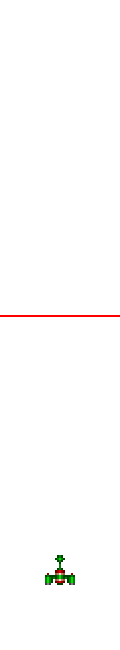
\includegraphics[scale=0.35]{fps_05e_120_00.png}}};
\node (fps240) at (8.0, 0) {\fbox{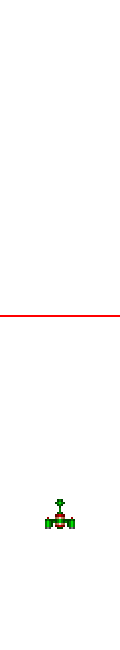
\includegraphics[scale=0.35]{fps_05e_240_00.png}}};
\node (fps300) at (10.0, 0) {\fbox{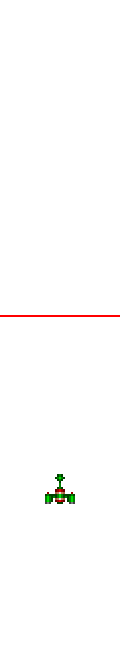
\includegraphics[scale=0.35]{fps_05e_300_00.png}}};
\node (fps600) at (12.0, 0) {\fbox{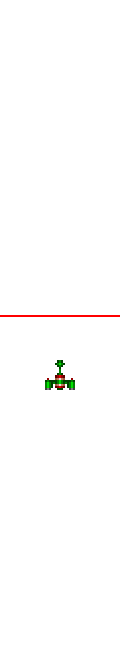
\includegraphics[scale=0.35]{fps_05e_600_00.png}}};
\end{tikzpicture}
	\caption[Nicht normalisierte Bewegung]{Nicht normalisierte Bewegung bei gleicher Geschwindigkeit aber unterschiedlichen Frameraten (von links nach rechts: 10, 30, 60, 120, 240, 300, 600)}\label{fpsbewegung00}
\end{center}
\end{figure}

\begin{longtable}{r@{ * }r@{ * }r@{ = }r}
	\caption{Strecke bei nicht normalisierter Geschwindigkeit}\label{tabFpsBewegung01} \\[1em]
	% Definition des Tabellenkopfes auf der ersten Seite
    Geschw. ($\frac{px}{f}$) & fps ($\frac{f}{s}$) & Zeit ($s$)& Strecke ($px$) \\[0.5em]\hline\hline
	\hline
	\endfirsthead % Erster Kopf zu Ende
	% Definition des Tabellenkopfes auf den folgenden Seiten
	\caption{Strecke bei nicht normalisierter Geschwindigkeit (Fortsetzung)}\\[1em]
	Geschw. ($\frac{px}{f}$) & fps ($\frac{f}{s}$) & Zeit ($s$)& Strecke ($px$)\\[0.5em]\hline\hline
	\hline
	\endhead % Zweiter Kopf ist zu Ende
	% Ab hier kommt der Inhalt der Tabelle
	2  &   10 & 0.5 &  10 \\ \hline
	2  &   30 & 0.5 &  30 \\ \hline
	2  &   60 & 0.5 &  60 \\ \hline
	2  &  120 & 0.5 & 120 \\ \hline
	2  &  240 & 0.5 & 240 \\ \hline
	2  &  300 & 0.5 & 300 \\ \hline
\end{longtable} 

Was wir also brauchen, ist eine Mechanismus, der die Framerate wieder rausrechnet. Dieser Faktor müsste so gebaut sein, dass er mit der Framerate multipliziert immer eine~1 als Ergebnis auswirft. Damit würde die Framerate im Gesamtprodukt wie eine Multiplikation mit~1 wirken, also keinen Einfluss mehr haben. Der naheliegende Weg wäre das Inverse der Framerate zu nehmen, also $\frac{1}{fps}$. Dieser Korrekturwert wird \emph{deltatime~(dt)}\index{deltatime}\randnotiz{deltatime} genannt. Die Berechnung würde dann beispielsweise wie in \tabref[vref]{tabFpsBewegung02} aussehen. Die zweite und die dritte Spalte heben sich auf, so dass die Strecke immer -- unabhängig von der gewählten Framerate -- gleich bleibt. 

\begin{longtable}{r@{ * }r@{ * }r@{ * }r@{ = }r}
	\caption{Strecke bei normalisierter Geschwindigkeit}\label{tabFpsBewegung02} \\[1em]
	% Definition des Tabellenkopfes auf der ersten Seite
    Geschw. ($\frac{px}{s}$) & fps ($\frac{f}{s}$) & dt ($\frac{s}{f}$) & Zeit ($s$) & Strecke ($px$) \\[0.5em]\hline\hline
	\hline
	\endfirsthead % Erster Kopf zu Ende
	% Definition des Tabellenkopfes auf den folgenden Seiten
	\caption{Strecke bei normalisierter Geschwindigkeit (Fortsetzung)}\\[1em]
	Geschw. ($\frac{px}{s}$) & fps ($\frac{f}{s}$) & dt ($\frac{s}{f}$) & Zeit ($s$) & Strecke ($px$)\\[0.5em]\hline\hline
	\hline
	\endhead % Zweiter Kopf ist zu Ende
	% Ab hier kommt der Inhalt der Tabelle
	2  &   10 &  $\frac{1}{10}$   & 0.5 &  1 \\ \hline
	2  &   30 &  $\frac{1}{30}$   & 0.5 &  1 \\ \hline
	2  &   60 &  $\frac{1}{60}$   & 0.5 &  1 \\ \hline
	2  &  120 &  $\frac{1}{120}$  & 0.5 &  1 \\ \hline
	2  &  240 &  $\frac{1}{240}$  & 0.5 &  1 \\ \hline
	2  &  300 &  $\frac{1}{300}$  & 0.5 &  1 \\ \hline
\end{longtable} 


In diesem Zusammenhang fällt auf, dass die Strecke erschreckend kurz ist: Nur~$1~px$ pro Sekunde. Bitte beachten Sie, dass sich auch die Maßeinheit der ersten Spalte geändert hat. Die Geschwindigeit gibt nun nicht mehr die Anzahl der Pixel pro Frame, sondern pro Sekunde an! Setzen wir daher eine andere Geschwindigeit fest; ich habe mich passend zu unserer Fenstgergröße mal für~$600~px/s$ entschieden. Nach einer Sekunde kommt unser Raumschiff also oben an. 

In \tabref[vref]{tabFpsBewegung03} habe ich mal berechnet, welche Endposition (\texttt{.top}) wir nach einer halben Sekunde erwarten können. In der linken Hälfte wird die Wegstrecke ausgerechnet. Überraschung: Sie beträgt immer $300~px$. Von der Fensterhöhe (\texttt{WINDOW.height}) müssen wir diese Wegstrecke abziehen. Ebenso die Höhe unseres Raumschiffs ($30~px$) und den kleinen Offset von $5~px$, da wir unser Raumschiff nicht ganz unten Rand starten lassen wollten. Wir erwarten also, dass unser Raumschiff nach einer halben Sekunde die in \tabref[vref]{tabFpsBewegung03} berechnete Endposition einnimmt.


\begin{longtable}{r@{ * }r@{ * }r@{ * }r@{ = }r@{ $\rightarrow$ }c@{ - }r@{ - }r@{ = }r}%{r@{ * }r@{ * }r@{ * }r@{ + }r@{ + }r@{ = }r@{ $\rightarrow$ }r}
	\caption{Pixelkoordinaten bei normalisierter Geschwindigkeit}\label{tabFpsBewegung03} \\[1em]
	% Definition des Tabellenkopfes auf der ersten Seite
    Geschw. & fps & dt  & Zeit  & Strecke & \texttt{WINDOW.height} & Höhe & Offset & \texttt{.top}\\[0.5em]\hline\hline
	\hline
	\endfirsthead % Erster Kopf zu Ende
	% Definition des Tabellenkopfes auf den folgenden Seiten
	\caption{Pixelkoordinaten bei normalisierter Geschwindigkeit (Fortsetzung)}\\[1em]
    Geschw. & fps & dt  & Zeit  & Strecke & \texttt{WINDOW.height} & Höhe & Offset & \texttt{.top}\\[0.5em]\hline\hline
	\hline
	\endhead % Zweiter Kopf ist zu Ende
	% Ab hier kommt der Inhalt der Tabelle
	600  &   10 &  $\frac{1}{10}$   & 0.5 & 300 & 650-300 & 30 & 5 & 315 \\ \hline
	600  &   30 &  $\frac{1}{30}$   & 0.5 & 300 & 650-300 & 30 & 5 & 315 \\ \hline
	600  &   60 &  $\frac{1}{60}$   & 0.5 & 300 & 650-300 & 30 & 5 & 315 \\ \hline
	600  &  120 &  $\frac{1}{120}$  & 0.5 & 300 & 650-300 & 30 & 5 & 315 \\ \hline
	600  &  240 &  $\frac{1}{240}$  & 0.5 & 300 & 650-300 & 30 & 5 & 315 \\ \hline
	600  &  300 &  $\frac{1}{300}$  & 0.5 & 300 & 650-300 & 30 & 5 & 315 \\ \hline
\end{longtable} 

\tabref{tabFpsBewegung03} sieht zwar kompliziert aus, die Umsetzung ist aber überraschend einfach. In \zeiref{srcInvader05f01} wird der Korrekturwert -- wie oben besprochen -- als Inverses von der Framerate definiert. Die Geschwindigkeit wird von~2 auf~600 in \zeiref{srcInvader05f02} angepasst und in \zeiref{srcInvader05f03} wird der Korrekturwert \texttt{DELTATIME} in Berechnung als Faktor eingebaut. Das war's; in \abbref[vref]{fpsbewegung01} können wir das \emph{perfekte} Ergebnis auf einem meiner langsameren Rechner bewundern. 

\lstsource{SRC/00 Einführung/04 Bewegung/invader05f.py}{7}{55}{python}{Normalisierte Bewegung mit $1/fps$}{srcInvader05f}

Zwei Probleme verursachen diese Fehler:

\begin{itemize}
    \item Rundungsfehler: Eigentlich sollte die Multiplikation der Framerate mit der Deltatime immer~$1.0$ ergeben. Das passiert leider aber nicht. Bei der Berechnung der Deltatime wird wegen des Formats einer \gls{float}\randnotiz{Rundungsfehler} ein Wert nahe des tatsächlichen Wertes abgespeichert; also beispielsweise bei $\frac{1.0}{30.0}$ nicht $0.0\overline{3}$, sondern $0.03333333333333330$. Dieser Rundungsfehler addiert sich im Laufe der Zeit zu wahrnehmbaren Größen auf.

    \item Falsches Verständnis von $fps$: Die Framerate definiert nicht, dass \emph{immer} die Hauptprogrammschleife beispielsweise 60 mal in der Sekunde durchlaufen wird, sondern dass sie \emph{maximal} 60 mal in der Sekunde durchlaufen wird. Nimmt die Spiellogik oder das Zeichnen der Oberfläche mehr Zeit in Anspruch als $1/60~s$, so wird mindestens ein Frame übersprungen. Dies tritt auch auf, wenn der Rechner durch andere Operationen (z.B. einer Cloud-Sync) Performance verliert. 
\end{itemize}

Das erste Problem können wir nicht ohne erheblichen Performaceverlust lösen und wird daher nicht weiter betrachtet. Das zweite Problem schon. Wir brauchen anstelle der festen Deltatime einen Wert, der sich aus der tatsächlichen Dauer eines Frames ergibt. Die Methode \texttt{pygame.clock.tick()}\myindex{pyg}{\texttt{clock}!\texttt{tick()}}\randnotiz{tick()} in \zeiref{srcInvader05g01} liefert mir nämlich eine gute Schätzung über die Laufzeit des Frames. Dieses Feature ist zum Glück schon eingebaut und kann daher einfach so verwendet werden (siehe \srcref[vref]{srcInvader05g}). Das Ergebnis in \abbref[vref]{fpsbewegung02} ist zwar besser aber trotzdem noch nicht befriedigend~{:-(}. In \abbref[vref]{picFehlerInvers} können Sie sehen, dass die rote Linie mehr oder weniger um die grüne herumtanzt und keine eindeutige Tendenz sichtbar ist.

\myebild{fehler_invers.pdf}{1.0}{Vergleich des Positionsfehlers von $1/fps$ und \texttt{pygame.clock.tick()}}{picFehlerInvers}

\newpage
\lstsource{SRC/00 Einführung/04 Bewegung/invader05g.py}{47}{52}{python}{Normalisierte Bewegung mit \texttt{pygame.clock.tick()}}{srcInvader05g}

Ursache ist ein Problem, welches wir hätten sofort lösen müssen. Bei der Zuweisung in \zeiref{srcInvader05f03} in \srcref[vref]{srcInvader05f} steht auf der rechten Seite eine Fließkommazahl\index{float} und auf der linken ein \gls{int}\index{int}. Dies führt dazu, dass die Nachkommastellen bei jedem Schleifendurchlauf abgeschnitten werden. Würde beispielsweise in jedem Frame das Raumschiff sich um $5.8~px$ bewegen müssen, entstünden diese Werte:

\begin{longtable}{lrrrrrrrrr}
	\caption{Fehlerfortpflanzung}\label{tabFpsBewegung04} \\[1em]
	% Definition des Tabellenkopfes auf der ersten Seite
    Frame & 1 & 2  & 3  & 4 & 5 &  6 & 7 & 8 & 9 \\[0.5em]\hline\hline
	\hline
	\endfirsthead % Erster Kopf zu Ende
	% Definition des Tabellenkopfes auf den folgenden Seiten
	\caption{Fehlerfortpflanzung (Fortsetzung)}\\[1em]
    Frame & 1 & 2  & 3  & 4 & 5 &  6 & 7 & 8 & 9 \\[0.5em]\hline\hline
	\hline
	\endhead % Zweiter Kopf ist zu Ende
	% Ab hier kommt der Inhalt der Tabelle
	Tatsächlicher Wert  & 5.0 & 10.0 & 15.0 & 20.0 & 25.0 & 30.0 & 35.0 & 40.0 & 45.0 \\ \hline
	Richtiger Wert      & 5.8 & 11.6 & 14.4 & 23.2 & 29.0 & 34.8 & 40.6 & 46.4 & 52.2 \\ \hline
	Fehler              & 0.8 & 1.3 & 2.4 & 3.2 & 4.0 & 4.8 & 5.6 & 6.4 & 7.2 \\ \hline
\end{longtable} 

Wir müssen die Positionswerte also unabhängig vom \texttt{Rect}-Objekt in einer zusätzlichen float-Variablen abspeichern, damit die Nachkommastellen erhalten bleiben. In \zeiref{srcInvader05h01} wird die aktuelle Position in einem \texttt{pygame.math.Vector2}\randnotiz{Vector2}\myindex{pyg}{\texttt{math}!\texttt{Vector2}|underline}-Objekt abgespeichert. Diese Klasse ist sehr gut dafür geeignet, Positionsangaben zu speichern. Mit Hilfe von \texttt{Vector2} und seinem Verwandten \texttt{pygame.math.Vector3}\randnotiz{Vector3}\myindex{pyg}{\texttt{math}!\texttt{Vector3}|underline} können Operationen wie Addition und Multiplikation einfacher implementiert werden. Mehr dazu später. 

\newpage
Auch werden die errechneten Positionswerte nicht einfach den Integer-Attributen des \texttt{Rect}-Objektes zugewiesen, sondern mit Hilfe von \texttt{round}\randnotiz{round()}\index{\texttt{round}} wird die Ganzzahl passend zu den Nachkommawerten nach den üblichen Rundungsregeln ermittelt (siehe \zeiref{srcInvader05h02}). 


\lstsource{SRC/00 Einführung/04 Bewegung/invader05h.py}{14}{57}{python}{Normalisierte Bewegung mit Positionsangaben in float}{srcInvader05h}

In \abbref[vref]{fpsbewegung03}  können wir sehen, dass das Ergebnis schon deutlich besser geworden ist. Auch hat sich die Abweichung von optimalen Wert~315 dramatisch verbessert. In \abbref[vref]{picFehlerFloat} wird der Unterschied sichtbar gemacht.

\myebild{fehler_float.pdf}{1.0}{Vergleich des Positionsfehlers ohne und mit Vector2}{picFehlerFloat}

Es gibt aber noch eine weitere Fehlerquelle: \texttt{pygame.clock.tick()}\myindex{pyg}{\texttt{clock}!\texttt{tick()}} liefert mir nicht genug Nachkommastellen. Bei langen Laufzeiten multipilizieren sich diese fehlenden Angaben nach vorne und führen wiederum zu Fehlern. Es gibt bessere Python-Funktionen zur Ermittlung von Laufzeiten.

In \zeiref{srcInvader05i01} von \srcref[vref]{srcInvader05i} wird mit Hilfe von \texttt{time.time()}\randnotiz{time()}\index{\texttt{time}!\texttt{time()}|underline} die Anzahl der Sekunden nach dem 01.01.1970 als eine Fließkommazahl (float) zurückgeliefert. Die Nachkommastellen geben dabei die Sekundenbruchteile an. Diese Messung ist genauer als die durch \texttt{pygame.clock.tick()} und liefert mir je nach Zeitmessungsmöglichkeiten der Rechnerarchitektur und des Betriebssystems mehr Nachkommastellen -- bis in den Nanosekundenbereich.

In \zeiref{srcInvader05i02} wird nach Ablauf eines Frame die aktuelle Zeit gemessen und in der Zeile danach der Zeitverbrauch ermittelt. Dieser ist dann die tatsächliche \emph{deltatime}\index{deltatime} des Frames, nun mit mehr Nachkommastellen. Anschließend wird in \zeiref{srcInvader05i04} dei neue Startzeit des nächsten Frames festgehalten, um nach dem nächsten Frame wieder den Zeitverbrauch ermitteln zu können.

\abbref[vref]{fpsbewegung04} zeigt uns, dass die Zielpositionen bei allen Frameraten nahezu perfekt getroffen wurden. Der Vergleich der Positionsfehler in \abbref[vref]{picFehlerFunktion} lässt aber keine eindeutige Bewertung zu. Ich denke mir aber, dass hier Experimente mit deutlich längeren Laufzeiten einen Unterschied erkennbar machen würden. Mit dem Restfehler müssen -- und können -- wir leben.

\myebild{fehler_funktion.pdf}{1.0}{Vergleich der Positionsfehler mit unterschiedlichen Genauigkeiten}{picFehlerFunktion}

\newpage 
\begin{figure}[p] 
	\begin{center}
		\begin{tikzpicture}
			\node (fps010) at (0.0, 0) {\fbox{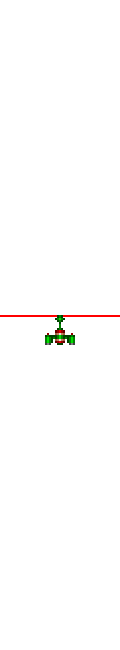
\includegraphics[scale=0.35]{fps_05f_010_00.png}}};
			\node (fps030) at (2.0, 0) {\fbox{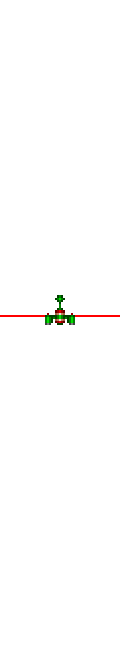
\includegraphics[scale=0.35]{fps_05f_030_01.png}}};
			\node (fps060) at (4.0, 0) {\fbox{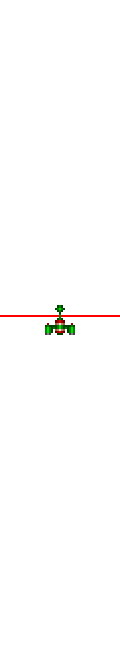
\includegraphics[scale=0.35]{fps_05f_060_02.png}}};
			\node (fps120) at (6.0, 0) {\fbox{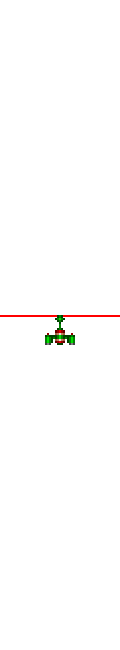
\includegraphics[scale=0.35]{fps_05f_120_09.png}}};
			\node (fps240) at (8.0, 0) {\fbox{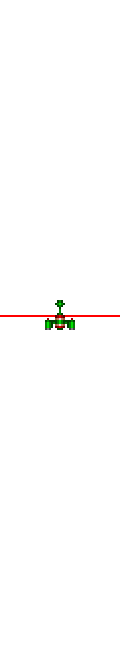
\includegraphics[scale=0.35]{fps_05f_240_04.png}}};
			\node (fps300) at (10.0, 0) {\fbox{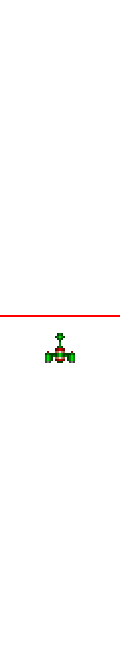
\includegraphics[scale=0.35]{fps_05f_300_09.png}}};
			\node (fps600) at (12.0, 0) {\fbox{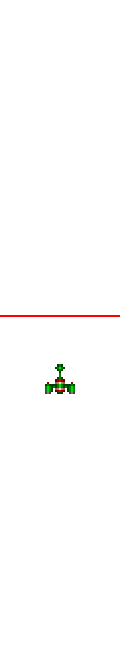
\includegraphics[scale=0.35]{fps_05f_600_09.png}}};
		\end{tikzpicture}
		\caption[Normalisierte Bewegung mit $1/fps$]{Normalisierte Bewegung mit $1/fps$ bei gleicher Geschwindigkeit aber unterschiedlichen Frameraten (von links nach rechts: 10, 30, 60, 120, 240, 300, 600)}\label{fpsbewegung01}
	\end{center}
\end{figure}


\begin{figure}[p] 
	\begin{center}
		\begin{tikzpicture}
			\node (fps010) at (0.0, 0) {\fbox{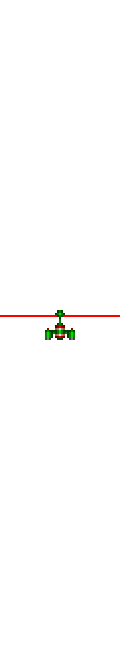
\includegraphics[scale=0.35]{fps_05g_010_08.png}}};
			\node (fps030) at (2.0, 0) {\fbox{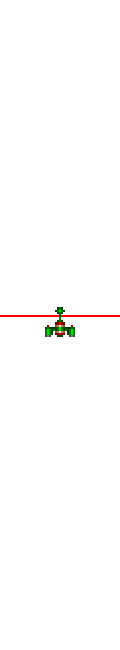
\includegraphics[scale=0.35]{fps_05g_030_07.png}}};
			\node (fps060) at (4.0, 0) {\fbox{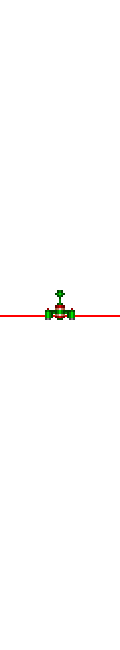
\includegraphics[scale=0.35]{fps_05g_060_05.png}}};
			\node (fps120) at (6.0, 0) {\fbox{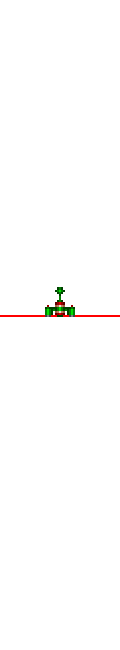
\includegraphics[scale=0.35]{fps_05g_120_04.png}}};
			\node (fps240) at (8.0, 0) {\fbox{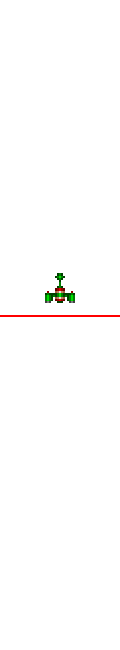
\includegraphics[scale=0.35]{fps_05g_240_08.png}}};
			\node (fps300) at (10.0, 0) {\fbox{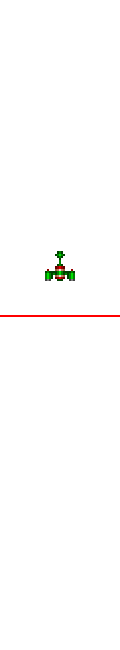
\includegraphics[scale=0.35]{fps_05g_300_08.png}}};
			\node (fps600) at (12.0, 0) {\fbox{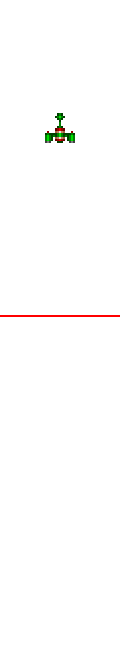
\includegraphics[scale=0.35]{fps_05g_600_06.png}}};
		\end{tikzpicture}
		\caption[Normalisierte Bewegung mit \texttt{pygame.clock.tick()}]{Normalisierte Bewegung  mit \texttt{pygame.clock.tick()} bei gleicher Geschwindigkeit aber unterschiedlichen Frameraten (von links nach rechts: 10, 30, 60, 120, 240, 300, 600)}\label{fpsbewegung02}
	\end{center}
\end{figure}

\newpage
\begin{figure}[p] 
	\begin{center}
		\begin{tikzpicture}
			\node (fps010) at (0.0, 0)  {\fbox{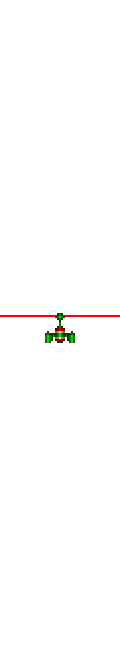
\includegraphics[scale=0.35]{fps_05h_010_09.png}}};
			\node (fps030) at (2.0, 0)  {\fbox{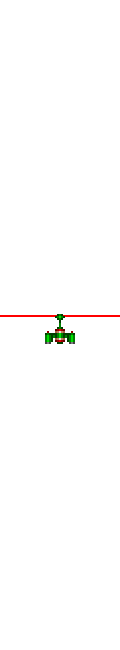
\includegraphics[scale=0.35]{fps_05h_030_05.png}}};
			\node (fps060) at (4.0, 0)  {\fbox{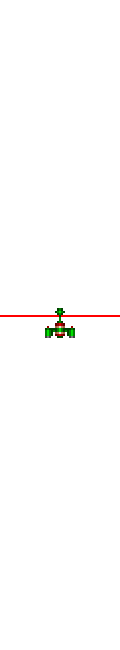
\includegraphics[scale=0.35]{fps_05h_060_05.png}}};
			\node (fps120) at (6.0, 0)  {\fbox{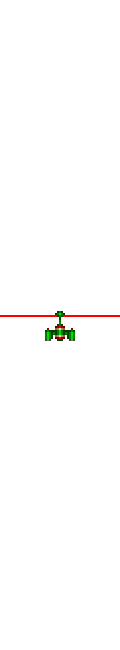
\includegraphics[scale=0.35]{fps_05h_120_04.png}}};
			\node (fps240) at (8.0, 0)  {\fbox{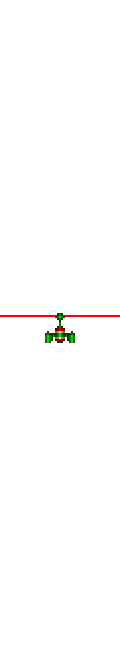
\includegraphics[scale=0.35]{fps_05h_240_05.png}}};
			\node (fps300) at (10.0, 0)  {\fbox{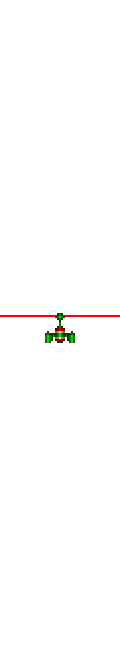
\includegraphics[scale=0.35]{fps_05h_300_06.png}}};
			\node (fps600) at (12.0, 0)  {\fbox{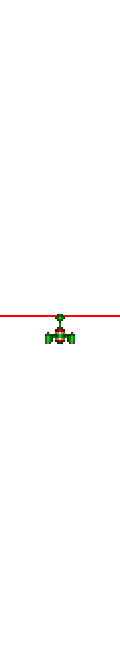
\includegraphics[scale=0.35]{fps_05h_600_09.png}}};
		\end{tikzpicture}
		\caption[Normalisierte Bewegung mit \texttt{pygame.clock.tick()} (float)]{Normalisierte Bewegung mit \texttt{pygame.clock.tick()} (float) bei gleicher Geschwindigkeit aber unterschiedlichen Frameraten (von links nach rechts: 10, 30, 60, 120, 240, 300, 600)}\label{fpsbewegung03}%
	\end{center}
\end{figure}

\begin{figure}[p] 
	\begin{center}
		\begin{tikzpicture}
			\node (fps010) at (0.0, 0) {\fbox{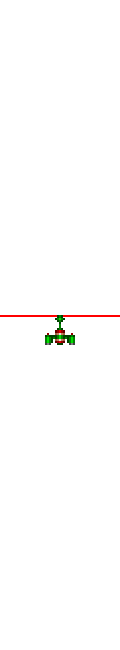
\includegraphics[scale=0.35]{fps_05i_010_00.png}}};
			\node (fps030) at (2.0, 0) {\fbox{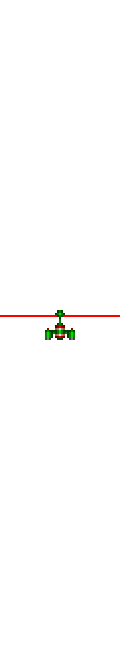
\includegraphics[scale=0.35]{fps_05i_030_05.png}}};
			\node (fps060) at (4.0, 0) {\fbox{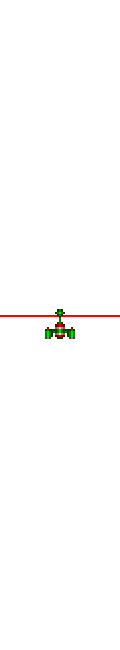
\includegraphics[scale=0.35]{fps_05i_060_03.png}}};
			\node (fps120) at (6.0, 0) {\fbox{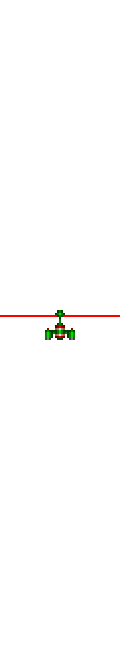
\includegraphics[scale=0.35]{fps_05i_120_07.png}}};
			\node (fps240) at (8.0, 0) {\fbox{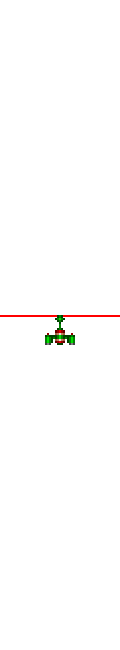
\includegraphics[scale=0.35]{fps_05i_240_00.png}}};
			\node (fps300) at (10.0, 0) {\fbox{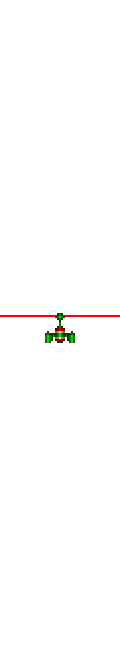
\includegraphics[scale=0.35]{fps_05i_300_00.png}}};
			\node (fps600) at (12.0, 0) {\fbox{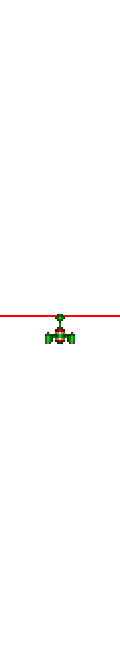
\includegraphics[scale=0.35]{fps_05i_600_00.png}}};
		\end{tikzpicture}
		\caption[Normalisierte Bewegung mit \texttt{time.time()}]{Normalisierte Bewegung mit \texttt{time.time()} bei gleicher Geschwindigkeit aber unterschiedlichen Frameraten (von links nach rechts: 10, 30, 60, 120, 240, 300, 600), Version 3}\label{fpsbewegung04}%
	\end{center}
\end{figure}
\newpage

\lstsource{SRC/00 Einführung/04 Bewegung/invader05i.py}{15}{60}{python}{Normalisierte Bewegung mit \texttt{time.time()}}{srcInvader05i}


%%%%%%%%%%%%%%%%%%%%%%%%%%%%%%%%%%%%%%%%%%%%%%%%%%%%%%%%%%%%%%%%%%%%%%%%%%%%%%%%
\subsection*{Was war neu?}
Die Position eines Objektes wird in einem \texttt{Rect}-Objekt abgelegt. In jedem Frame wird die Position überprüft und ggf. verändert. Bei einer Bildschirmausgabe entsteht dadurch der Eindruck einer Bewegung. Das Ergebnis einer Bewegung wird in der Regel zunächst in einer Variablen zwischengespeichert und überprüft, bevor es zur Positionsänderung verwendt wird.

Die Bewegungsrichtung wird durch das Vorzeichen und die Geschwindigkeit durch den Wert der Geschwindigkeitsvariablen kodiert. Dabei werden die horizontale und vertikale Richtung getrennt verarbeitet.

Um unabhängig von der tatsächlichen Framerate zu werden, muss bei der Berechnung der neuen Position ein Korrekturwert (Deltatime) verwendet werden. Dieser kann selbst berechnet werden oder aus dem Aufruf von \texttt{pygame.time.Clock.tick()} verwendet werden.

Das Rechteck des Bitmaps speichert seine Werte als Ganzzahlen ab. Dadurch gehen die Nachkommastellen verloren und führen zu Positionsfehlern. Parallel zum Rechteck sollte daher ein \texttt{Vector2}-Objekt zur Speicherung der Positionskoordinaten verwendet werden. Dieses speichert die Werte als Fließkommazahlen ab.

Es wurden folgende Pygame-Elemente eingeführt:

\begin{itemize}

	\item \texttt{pygame.Rect}:
	\myindex{pyg}{\texttt{Rect}}\\
	\url{https://www.pygame.org/docs/ref/rect.html}
	
	\item \texttt{pygame.Rect.move()}:
    \myindex{pyg}{\texttt{Rect}!\texttt{move()}}\\
    \url{https://www.pygame.org/docs/ref/rect.html#pygame.Rect.move}

	\item \texttt{pygame.Surface.get\_rect()}:
	\myindex{pyg}{\texttt{Surface}!\texttt{get\_rect()}}\\
	\url{https://www.pygame.org/docs/ref/surface.html#pygame.Surface.get_rect}

	\item \texttt{pygame.time.get\_ticks()}:
    \myindex{pyg}{\texttt{time}!\texttt{get\_ticks()}}\\
    \url{https://www.pygame.org/docs/ref/surface.html#pygame.time.get_ticks}

    \item \texttt{pygame.math.Vector2}:
    \myindex{pyg}{\texttt{math}!\texttt{Vector2}}\\
    \url{https://www.pygame.org/docs/ref/math.html#pygame.math.Vector2}

    \item \texttt{pygame.math.Vector3}:
    \myindex{pyg}{\texttt{math}!\texttt{Vector3}}\\
    \url{https://www.pygame.org/docs/ref/math.html#pygame.math.Vector3}
\end{itemize}

